\chapter{Background}\label{ch:background}
\graphicspath{{../Figures/15-background/}{figs/15-background/}}

This chapter reviews the established knowledge against which the dissertation's contributions are defined: biomimetic and musculoskeletal robotics, the actuation technologies available to them, the human lower-limb biomechanics they imitate, the neuroscience of locomotor control they implement, and the simulation and ethical context in which they are tested. Work from my own program that goes beyond this background, including the prior AnimatLab bipedal walker, the Sensory Afferent Database, and the neuromechanical simulation pipeline, is presented as dissertation work in Chapters~\ref{ch:database} and~\ref{ch:sns} rather than repeated here.

\section{Biomimetic and Musculoskeletal Robots}\label{sec:bg_robots}

Biomimetic robots offer many potential applications, ranging from assisting in factories and environmental exploration to serving as physical models of human movement. By developing high-fidelity biomimetic robots, we can perform tests that help improve our understanding of both biomechanics and the underlying neuromechanical systems that control movement \citep{shin_constructive_2018, asano_musculoskeletal_2019, ijspeert_amphibious_2020, goldsmith_investigating_2021, hunt_development_2017, schilling_adaptive_2022}. A few such biomimetic robots exist, such as the impressive Kengoro and Kenshiro robots of \citet{asano_design_2017} and \citet{asano_musculoskeletal_2019}, which have proportionally human bodies, anatomically correct musculotendon arrangements, rolling-sliding joints, and joint ranges and output power comparable with human-measured values; their artificial muscles are implemented with brushless DC motors, wires as tendons, gears, and integrated tension measurement. Kengoro, the more recent of the two, stands \qty{1670}{\mm} tall, weighs \qty{56.5}{\kg}, and carries 174 degrees of freedom when the end effectors are included \citep{asano_design_2017}. A dog-like robot developed by \citet{aschenbeck_design_2006} and actuated with Festo BPAs was designed from a planar kinematic model scaled to an adult greyhound, with three sagittal degrees of freedom per leg driven by antagonistic BPA pairs; its front-leg pair alone lifted a \qty{13.5}{\kg} payload, almost double the complete robot's predicted mass. That platform was used to show how central pattern generators provide robust locomotion patterns that are adaptive to perturbations in ground speed \citep{hunt_development_2017}.

Robots built with artificial muscles thus provide opportunities to investigate how muscles are controlled to produce desired motions; however, artificial muscles do not exactly replicate muscle properties, and existing robots do not capture all of the degrees of freedom and joint torques of the animal limbs they mimic. The biomimetic leg developed and tested in this dissertation sits squarely in this lineage: a human-proportioned skeleton, muscle-like actuators, and the goal of human-matched joint torques.

Figure~\ref{fig:kengoro_humanoid} illustrates the human-scale skeletal structure and tendon routing of this approach.

\begin{figure}[htbp]
\centering
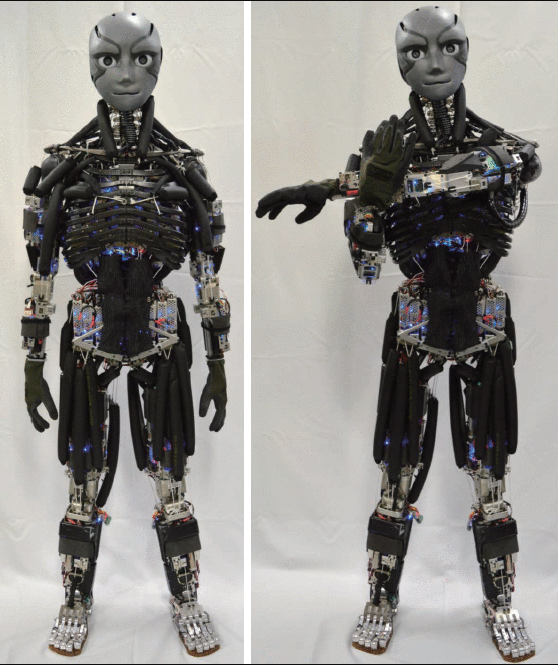
\includegraphics[width=0.78\textwidth]{kengoro_humanoid_comparison.png}
% ALT TEXT: Two frontal views of the Kengoro humanoid show its human-scale
% skeletal frame, dense tendon routing, and musculoskeletal construction.
\caption[Kengoro human-mimetic musculoskeletal humanoid]{Kengoro human-mimetic musculoskeletal humanoid in neutral and upper-limb poses, illustrating its human-scale skeletal structure and densely routed tendon-driven musculature \citep{asano_design_2017}.}
\label{fig:kengoro_humanoid}
\end{figure}


\section{Robot Actuation Technologies}\label{sec:bg_actuation}

\subsection{Overview}\label{sec:bg_actuation_overview}

A wide range of actuation technologies have been explored in robotics, including electric motors, hydraulic systems, smart-material actuators, and artificial muscles \citep{he_mechanism_2020, liang_comparative_2020}. Electric motors are widely used due to their controllability and maturity, but they are limited by thermal constraints, gearing requirements, and reduced compliance compared to muscle-like actuators \citep{veale_towards_2016, suzumori_trends_2018}. Hydraulic actuators offer exceptionally high power density and have enabled highly dynamic legged systems, but they remain relatively heavy, less efficient than biological muscle, and require a dedicated fluid infrastructure \citep{suzumori_trends_2018}.

Among smart-material actuators, dielectric elastomer actuators (DEAs), a class of electronic electroactive polymers, contract by a different mechanism: an applied voltage squeezes a soft polymer film between compliant electrodes through electrostatic stress, and the thinning and radial spreading of the film produces strains that can exceed biological muscle \citep{madden_artificial_2004}. Comparative studies report high specific work and good bandwidth for DEAs \citep{liang_comparative_2020}, but kilovolt-range driving voltages, electromechanical instability, and the compliant-electrode requirement have kept them out of legged robots. Thermally activated artificial muscles reach the most extreme performance figures of any technology surveyed by \citet{liang_comparative_2020}: twisted-fiber muscles support loads more than one hundred times those of a biological muscle of the same length and weight, with output stresses of \qty{22}{\mega\pascal}. Their activation route, however, is shared with shape-memory alloys, whose heating is fast but whose cooling is limited by heat transfer away from the element, and that asymmetry sets the cycle time.

Closer to muscle, series-elastic and pneumatic actuators trade peak force and bandwidth for compliance, a trade that wearable and rehabilitation robotics exploit because force control and backdrivability matter most when a machine interacts with a human \citep{aksoz_design_2019, leibach_development_2020, li_influence_2020}. A recent review of pneumatic artificial muscle technology documents continued progress in actuator design and in assistive applications \citep{zhagiparova_recent_2025}. None of these technologies yet combines muscle-like force, strain, and compliance in one actuator, which is the combination a biomimetic humanoid leg demands and that braided pneumatic actuators approximate most closely.

Figure~\ref{fig:actuator_technology_comparison} compares the operating mechanisms of these actuator technologies.

\begin{figure}[htbp]
\centering
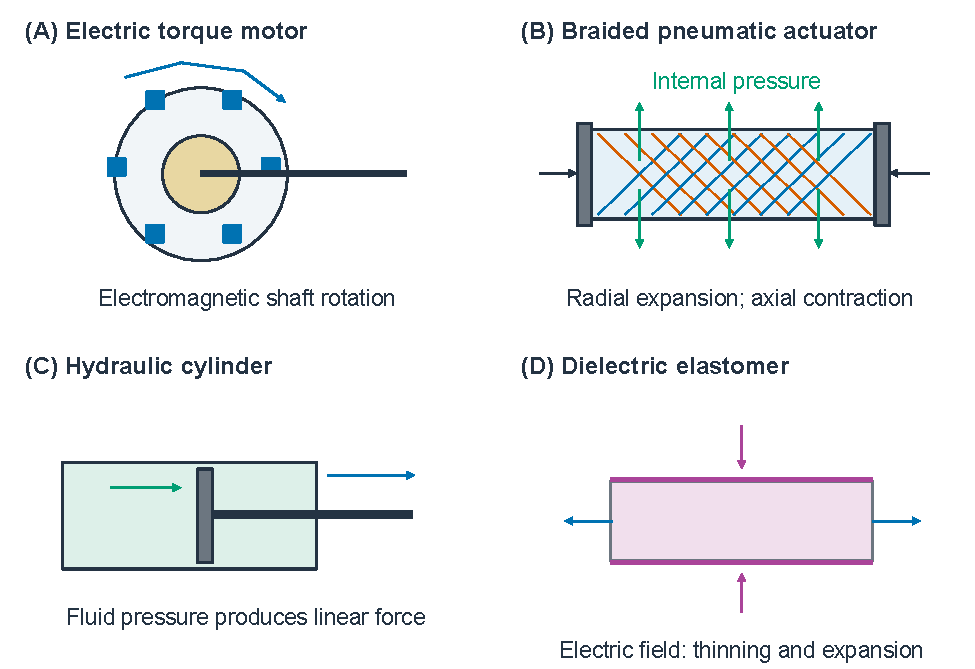
\includegraphics[width=0.96\textwidth]{actuator_technology_comparison.pdf}
% ALT TEXT: Four schematic panels compare an electric torque motor, a braided
% pneumatic actuator, a hydraulic cylinder, and a dielectric elastomer actuator.
% Arrows show each device's characteristic motion or applied pressure or voltage.
\caption[Representative robotic actuator technologies]{Representative operating mechanisms for robotic actuators. \textbf{(A)} An electric torque motor produces controlled shaft rotation. \textbf{(B)} A braided pneumatic actuator shortens as internal pressure expands its sleeve radially. \textbf{(C)} A hydraulic cylinder converts fluid pressure into linear piston force. \textbf{(D)} A dielectric elastomer thins and expands laterally under an applied electric field. The panels use a consistent schematic style to emphasize the distinct energy-conversion mechanisms and design tradeoffs summarized in the text \citep{suzumori_trends_2018, liang_comparative_2020}.}
\label{fig:actuator_technology_comparison}
\end{figure}

\subsection{Braided Pneumatic Actuators}\label{sec:bg_bpa}

In contrast to the technologies above, McKibben-style braided pneumatic actuators (BPAs) combine low mass, high force-to-weight ratio, and intrinsic compliance with a force--length curve that qualitatively resembles that of skeletal muscle \citep{liang_comparative_2020, hunt_modeling_2017}. A BPA consists of an inflatable bladder inside a braided sleeve; pressurizing the bladder expands the bladder radially and contracts the sleeve axially, producing tensile force. As shown by Chou and Hannaford, the force--length relationship of McKibben actuators is governed by geometric constraints imposed by the braided shell, leading to a nonlinear dependence of force on actuator length through the braid angle \citep{chou_measurement_1996}: actuator force is proportional to pressure and to a nonlinear geometric term $(3\cos^2\theta - 1)$, which governs both the maximum contraction limit and the curvature of the force--length relationship. Predicting their force as a function of length and pressure is therefore the first improvement of the torque tools developed in this dissertation, and the state of that prediction is the subject of the next subsection.

Figure~\ref{fig:festo_bpa_cad} shows the commercial actuator assembly used in the laboratory.

\begin{figure}[htbp]
\centering
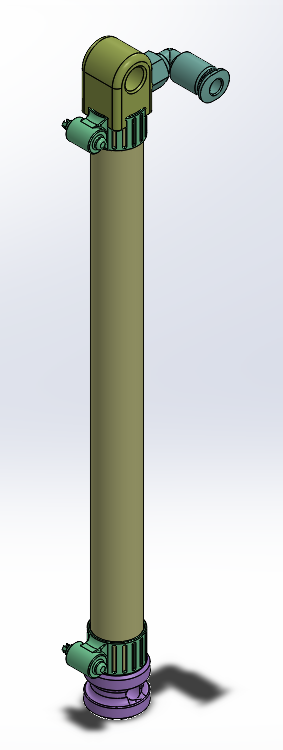
\includegraphics[height=0.45\textheight,keepaspectratio]{festo_bpa_cad.png}
% ALT TEXT: A vertical CAD rendering shows a Festo braided pneumatic actuator
% with its long cylindrical muscle body, end fittings, mounting hardware, and
% pneumatic connections.
\caption[Festo braided pneumatic actuator assembly]{CAD representation of a Festo DMSP braided pneumatic actuator with the mounting and pneumatic connections used in the laboratory assembly \citep{festo_2026}. The long cylindrical body contains the bladder and braided sleeve; pressurization through the end fittings converts radial expansion into axial contraction.}
\label{fig:festo_bpa_cad}
\end{figure}

However, BPAs exhibit several important differences from biological muscle. First, BPA maximum tensile force occurs at resting (i.e., uninflated) length ($l_0$) rather than at an optimal fiber length \citep{liang_comparative_2020}. Second, their maximum contraction ratio is substantially lower than that of human muscle, presenting challenges for achieving biomimetic joint ranges of motion \citep{hunt_modeling_2017, sarosi_comparative_2017, liang_comparative_2020}. Third, BPAs have a highly nonlinear dependence on internal pressure ($P$), contraction ($\epsilon$), and loading state \citep{hunt_modeling_2017, martens_modeling_2017}, which complicates control and motivates high-fidelity force--length--pressure modeling. Despite these differences, their muscle-like properties have made them attractive for biomimetic quadrupeds \citep{aschenbeck_design_2006, scharzenberger_design_2019}, humanoids \citep{asano_design_2017, hitzmann_anthropomorphic_2018}, and musculoskeletal arms \citep{kurumaya_musculoskeletal_2016, chen_realizing_2019}.

\subsection{BPA Force--Length--Pressure Models}\label{sec:bg_bpamodels}

Previous studies have generated empirical models of the force--length--pressure relationship of BPAs. \citet{sarosi_comparative_2017} discuss several high-fidelity BPA force models. They present a static force model with a 21-coefficient polynomial function for a Festo MAS-20-200N (i.e., $\diameter$\qty{20}{\mm}, $l_0=\qty{200}{\mm}$) with an impressive $\text{R}^2=0.9994$, as well as S\'arosi's static force model for a Festo DMSP-20-400N-RM-RM (i.e., $\diameter$\qty{20}{\mm}, $l_0=\qty{400}{\mm}$), with six coefficients and a $\text{R}^2=0.9995$ \citep{sarosi_new_2012, sarosi_investigation_2013}. Martens and Boblan present an even more accurate model, in terms of absolute error, using five coefficients for a DMSP-10-250 (i.e., $\diameter$\qty{10}{\mm}, $l_0=\qty{250}{\mm}$) and a DMSP-20-300 (i.e., $\diameter$\qty{20}{\mm}, $l_0=\qty{300}{\mm}$) \citep{martens_modeling_2017}. However, as demonstrated in this work, different resting lengths produce different force--length curves, preventing the use of these single-length models for designing systems with different resting lengths.

\citet{hunt_modeling_2017} looked at six resting lengths of $\diameter$\qty{10}{\mm} Festo BPAs, accounting for differences in maximum contractile percentages, and elucidated the force-length-pressure relationship. In particular, for a given contraction percent and force $F$ (in Newtons), the scalar pressure $P$ (in kPa) required to produce this force for a $\diameter$\qty{10}{\mm} Festo artificial muscle can be determined by solving the equation:

\begin{equation}
P = P_{0} + k_{F}\,F + k_{S}\,S + P_{t}\tan\!\left(c_{a}\left[\frac{\epsilon}{\epsilon_{\max} - k_{E}\,F} - c_{b}\right]\right) \label{eq:BPAFit}
\end{equation}

\noindent
where $F$ is the required force, $\epsilon$ is the contraction, $S$ encodes hysteresis ($S=1$ shortening, $S=-1$ lengthening, $S=0$ static), and the seven coefficients are defined in Table~\ref{tab:BPAFit_coeff}. The coefficients have been updated with corrected values, as those reported in \citet{hunt_modeling_2017} contained typographical errors. The contraction $\epsilon$ and the maximum free-load contraction at \qty{620}{\kPa}, which appears as $\epsilon_{\max}$ in Equation~(\ref{eq:BPAFit}), are defined in Section~\ref{sec:force_model}, together with the relative contraction $\epsilon^{*} = \epsilon/\epsilon_{620}$ on which the force surface developed in this dissertation is built. Because Equation~(\ref{eq:BPAFit}) expresses pressure in closed form as a function of force and contraction, it can also be solved onto a grid of pressures and contractions to build a force--pressure--relative-contraction lookup table for design studies.

\begin{table}[htbp]
\centering
\caption{Coefficients of the \qty{10}{\mm} Festo BPA pressure model of Equation~(\ref{eq:BPAFit}), corrected from \citet{hunt_modeling_2017}.}
\label{tab:BPAFit_coeff}
\begin{tabular}{lll}
\hline
Symbol & Value & Role \\
\hline
$P_{0}$ & \qty{254}{\kPa} & pressure offset \\
$k_{F}$ & \qty{1.23}{\kPa\per\newton} & linear force-to-pressure gain \\
$k_{S}$ & \qty{15.6}{\kPa} & hysteresis offset (sign of $S$) \\
$P_{t}$ & \qty{192}{\kPa} & tangent-term amplitude \\
$c_{a}$ & 2.03 & contraction-shape coefficient \\
$c_{b}$ & 0.46 & contraction-shift coefficient \\
$k_{E}$ & \qty{0.331e-3}{\per\newton} & force-dependent reduction of usable contraction \\
\hline
\end{tabular}
\end{table}

Festo provides a manufacturer tool, MuscleSIM, for predicting force as a function of pressure and contraction \citep{lang_robert_musclesim_2005}, but experimental comparisons indicate that it does not adequately account for variation in $l_0$ or actuator-specific contraction limits. Comparisons with experimental data indicate that none of the existing models effectively take into account differences in maximum force due to initial actuator length, and the Hunt model was taken with low external forces ($\leq$\qty{106}{\newton}), so it is unclear how well it captures actuator behavior at higher forces. Chapter~\ref{ch:muscles} compares these models with data collected for this dissertation and develops the improved characterization on which the torque and controller work of the later chapters depends.

\section{Human Lower-Limb Biomechanics}\label{sec:bg_biomechanics}

Designing a biomimetic leg requires a quantitative benchmark of human muscle--joint behavior. This dissertation uses OpenSim \citep{delp_opensim_2007, seth_opensim_2011, seth_opensim_2018} and the Gait2392 model, named for its 23 degrees of freedom and 92 musculotendon actuators. Gait2392 descends from the interactive lower-extremity model of \citet{delp_interactive_1990} and includes musculoskeletal geometry from \citet{hoy_musculoskeletal_1990} and planar knee kinematics from \citet{yamaguchi_planar_1989}; related lower-limb models of the same family are characterized and validated by \citet{arnold_model_2010}. Muscle moment arms, force-generating properties, and functional roles in such models have been characterized extensively \citep{zajac_determining_1989, brand_model_1982, menegaldo_moment_2004, millard_flexing_2013, sherman_what_2013, suderman_moving_2012}, and standard reporting conventions for kinematics and joint mechanics are established by the International Society of Biomechanics \citep{wu_for_1995, wu_isb_2002, wu_isb_2005, derrick_isb_2020}.

Moment arms relate muscle force to joint torque. For a fixed-axis joint, the signed moment arm is $r_{\mathrm{m}}=\hat{\mathbf{a}}\cdot(\mathbf{r}\times\hat{\mathbf{u}})$, where $\hat{\mathbf{a}}$ is the joint-axis direction, $\mathbf{r}$ locates a point on the muscle's line of action relative to the joint, and $\hat{\mathbf{u}}$ is the force direction \citep{brand_model_1982}. The tendon-excursion method instead evaluates the sensitivity of musculotendon length to the joint coordinate, with sign determined by the coordinate and force conventions \citep{menegaldo_moment_2004}. For multiarticular muscles, the result also depends on adjacent-joint configurations \citep{zajac_determining_1989, young_analyzing_2019}. OpenSim uses length sensitivities, so the reference moment arms in this dissertation are properties of the Gait2392-derived geometry \citep{delp_opensim_2007, seth_opensim_2018}. Chapter~\ref{ch:torque} compares the robot's resulting torque predictions with test-stand measurements.

Knee modeling requires particular care because the instantaneous center of rotation changes with flexion. Four-bar descriptions reproduce this behavior through linkage geometry \citep{romero_four-bar_2020, steele_biomimetic_2018}. Gait2392 instead prescribes planar translations as functions of knee flexion \citep{yamaguchi_planar_1989}. These different kinematics produce different moment arms for the same nominal attachment locations. Joint-coordinate conventions must therefore be stated consistently when comparing models and measurements \citep{wu_isb_2002}. Gait2392 provides the human reference in this dissertation, while Steele's four-bar mechanism supplies the physical robot knee.

\section{Biomimetic Knee and Bipedal Robot Model}\label{sec:bg_knee}

Steele's biomimetic knee joint supplies the physical knee used in this dissertation \citep{steele_development_2017, steele_biomimetic_2018, steele_biomimetic_2018-1}. It is a one-degree-of-freedom four-bar linkage whose crossed links reproduce the posterior migration of the human knee's instantaneous center of rotation (ICR) during flexion. The rolling-and-sliding behavior of the human joint therefore emerges from the link geometry itself rather than from cams or gear profiles, and the design was calculated to reproduce an average sliding-to-rolling ratio of 0.079 over a \ang{151} range of motion \citep{steele_biomimetic_2018-1}. Because the ICR migrates, muscle moment arms about the knee change with flexion angle in a human-like way, and a torque prediction tool for this knee must capture that variation rather than assume a constant arm. The biomimetic knee tests of Chapter~\ref{ch:torque} therefore exercise the corrected torque model against this geometry, and Figure~\ref{fig:steele_knee} summarizes the mechanism.

\begin{figure}[htbp]
\centering
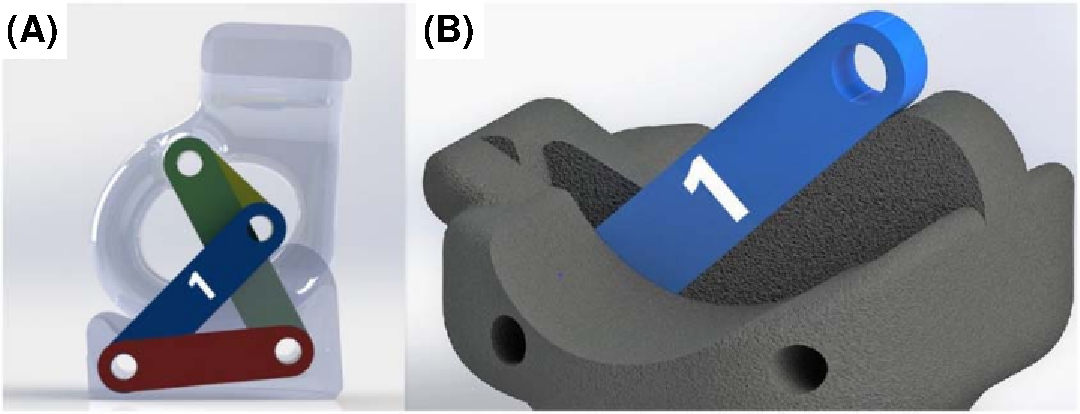
\includegraphics[width=0.95\textwidth]{steeleknee.pdf}
% ALT TEXT: Two panels reproduced from Steele et al. Figure 6. Panel (a) is a
% sagittal cutaway of the biomimetic knee at full extension, showing the crossed
% four-bar linkage. Panel (b) is an exploded view of the knee's mechanical stop.
\caption[Steele biomimetic knee mechanism]{Biomimetic knee mechanism. \textbf{(a)} Sagittal cutaway at full extension showing the crossed four-bar linkage. \textbf{(b)} Exploded view of the mechanical stop. Reproduced from \citet[Fig.~6]{steele_biomimetic_2018-1} under CC BY 4.0.}
\label{fig:steele_knee}
\end{figure}

In my master's work, muscle lengths, moment arms, and isometric joint torques were computed over the range of motion for both the Gait2392 model and a PAM-actuated robot leg model, demonstrating that several robot muscle torque profiles could closely match the human model while many fell far short for part of the RoM \citep{bolen_bipedal_2019, bolen_determination_2019}. Hand placement of muscle origins and insertions was a painstaking and iterative task. This resulted in the creation of a placement optimization algorithm \citep{morrow_optimization_2020}, discussed in Chapter~\ref{ch:torque}. Figure~\ref{fig:aarl_opensim_comparison} shows the two sides of that comparison: the laboratory's bipedal skeleton and the OpenSim muscle-routing reference developed for it.

\begin{figure}[htbp]
\centering
\begin{minipage}[c]{0.67\textwidth}
\centering
\textbf{(A)}\par\smallskip
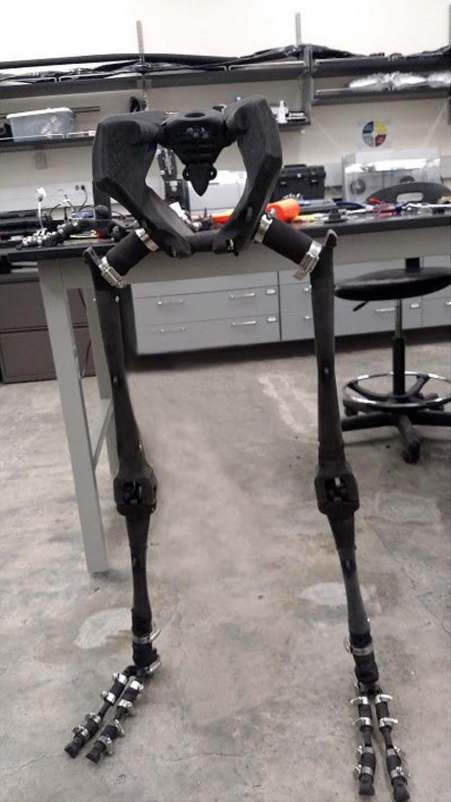
\includegraphics[width=\linewidth,height=0.52\textheight,keepaspectratio]{aarl_bpa_biped.png}
\end{minipage}\hfill
\begin{minipage}[c]{0.25\textwidth}
\centering
\textbf{(B)}\par\smallskip
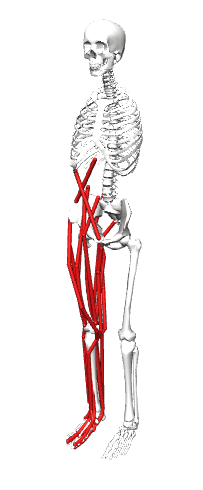
\includegraphics[width=\linewidth]{gait2392_27_muscle_model.png}
\end{minipage}
% ALT TEXT: (A) The laboratory bipedal skeleton, shown without actuators
% installed. (B) A Gait2392-derived OpenSim model shows the retained
% lower-limb muscle paths in red beside the skeletal geometry.
\caption[Laboratory biped skeleton and OpenSim muscle model]{\textbf{(A)} The laboratory biped skeleton (actuators not installed in this view). \textbf{(B)} The Gait2392-derived OpenSim model used to develop its muscle routing; the view exposes the retained lower-limb musculotendon paths used as biomechanical design references \citep{bolen_determination_2019, morrow_optimization_2020}.}
\label{fig:aarl_opensim_comparison}
\end{figure}

The comparison evaluated muscle-path lengths, moment arms, and isometric torques across the human and robot models \citep{bolen_bipedal_2019}. I adjusted BPA origins, insertions, and via-point locations to respect usable contraction and avoid interference. The biceps femoris long head illustrates the remaining mismatch: the robot path and its knee- and hip-torque surfaces differ substantially from the human reference. These discrepancies motivated placement optimization \citep{morrow_optimization_2020}. Figures~\ref{fig:masters_routing_and_arms} and~\ref{fig:masters_torque_comparison} show the geometry and the torque comparison.

\begin{figure}[htbp]
\centering
\textbf{(A)}\par\smallskip
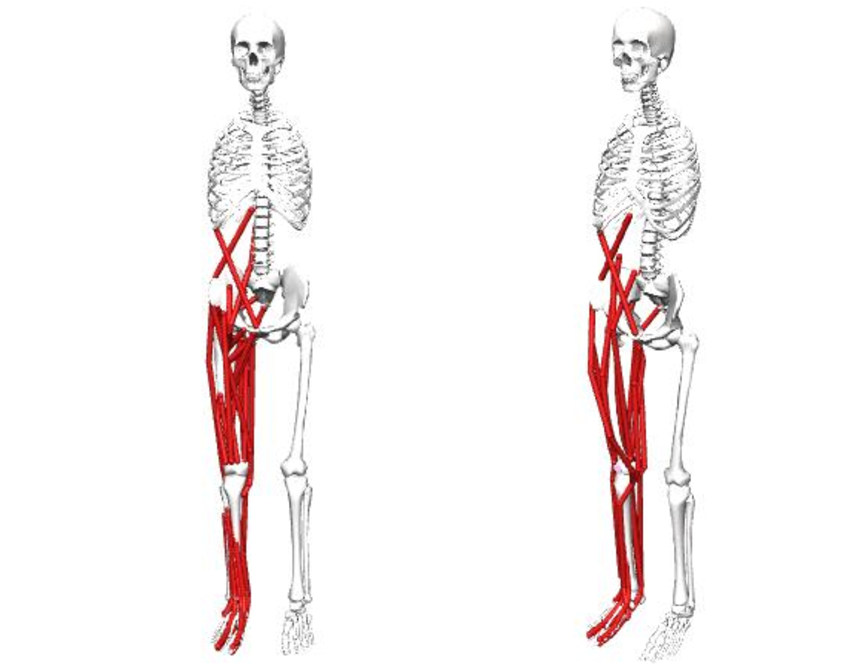
\includegraphics[width=0.72\textwidth]{masters_leg_model.pdf}\par\medskip
\textbf{(B)}\par\smallskip
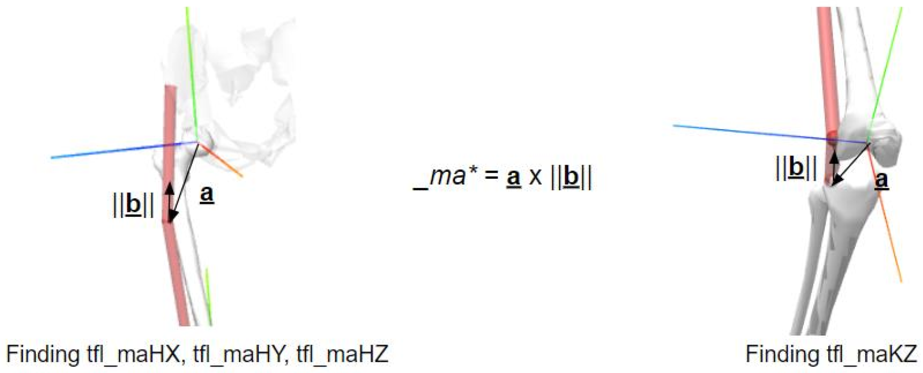
\includegraphics[width=0.92\textwidth]{masters_moment_arm.pdf}
% ALT TEXT: (A) Two anterior OpenSim renderings: the human skeleton with
% Gait2392 muscle paths and the robot leg skeleton with PAM paths. (B) Two
% model renders with the cross-product construction of a muscle moment arm
% about hip axes and the knee axis.
\caption[Master's-study routing models and moment-arm construction]{Master's-study geometry. \textbf{(A)} Human Gait2392 muscle paths and robot PAM routes. \textbf{(B)} Geometric constructions used to evaluate moment arms about the hip and knee \citep[Figs.~4 and~6]{bolen_bipedal_2019}.}
\label{fig:masters_routing_and_arms}
\end{figure}

\begin{figure}[htbp]
\centering
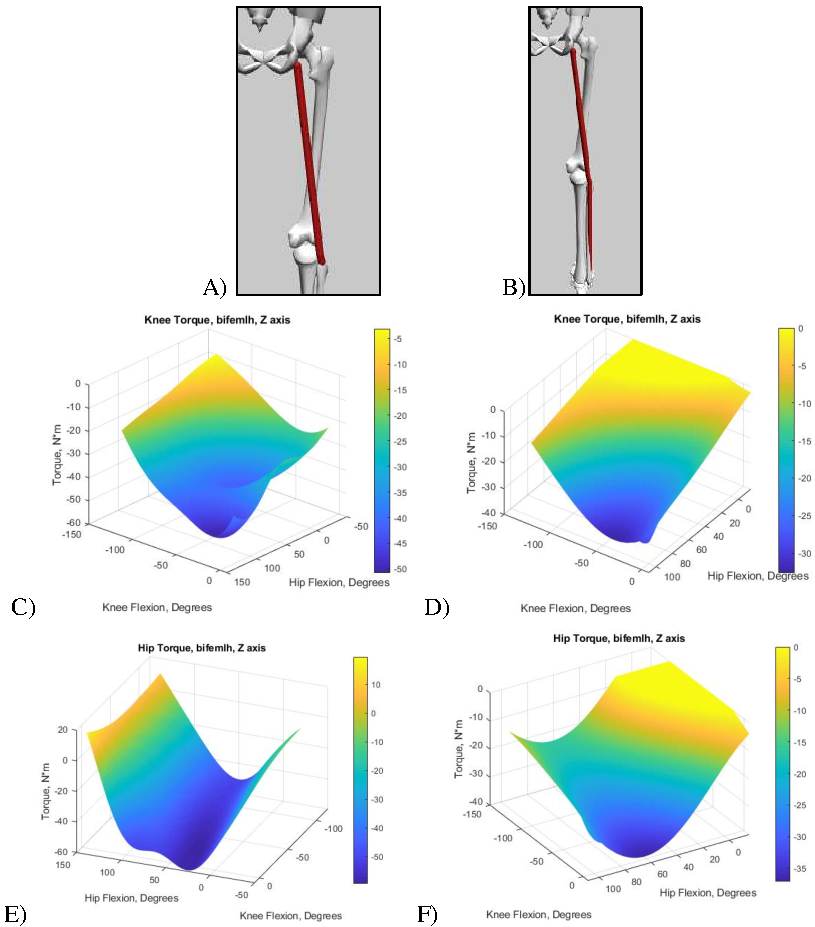
\includegraphics[width=0.62\textwidth]{masters_torque_comparison.pdf}
% ALT TEXT: Six panels: biceps femoris long-head muscle paths in the human
% and robot models, and four 3D isometric torque surfaces comparing knee and
% hip-axis torque between the models.
\caption[Biceps femoris long-head torque comparison from the master's study]{Biceps femoris long head in the master's study: muscle paths in the OpenSim model (A, C, E) and the robot model (B, D, F), with isometric torque surfaces about the knee (C, D) and the hip axis (E, F) over the hip--knee range \citep[Fig.~8]{bolen_bipedal_2019}.}
\label{fig:masters_torque_comparison}
\end{figure}

\section{Neural Control of Locomotion: Central Pattern Generators}\label{sec:bg_neural}

Locomotion in mammals is driven by spinal central pattern generators (CPGs), neural circuits that can produce alternating rhythmic activity of flexor and extensor motoneurons in the absence of rhythmic input and proprioceptive feedback \citep{brown_intrinsic_1911, rybak_modelling_2006}. The founding hypothesis is Brown's half-center: alternating flexor and extensor activity arises from two reciprocally inhibitory central populations with opposing bias \citep{brown_intrinsic_1911}. Modern instantiations of the half-center endow each neuron with persistent sodium channels, whose slow inactivation terminates each burst so that reciprocal inhibition switches the populations without any phasic input \citep{deng_neuromechanical_2019}; rhythmogenesis, in this tradition, is a property of the intrinsic membrane dynamics, not of a clock elsewhere in the network. The modern architectural understanding of mammalian locomotor CPGs comes largely from the modeling work of the Rybak group and collaborators. \citet{rybak_modelling_2006} proposed that the locomotor CPG consists of two levels: a half-center rhythm generator (RG) and a pattern formation (PF) network, with reciprocal inhibitory interactions between antagonist neural populations at each level. This two-level organization explains, among other phenomena, spontaneous deletions of motoneuron activity during fictive locomotion in which the locomotor period and phase are maintained, and it permits independent control of the level of motoneuron activity and of step-cycle timing. \citet{mccrea_organization_2008} reviewed the electrophysiological support for this organization, and \citet{rybak_organization_2015} related the model architecture to genetically identified spinal interneuron classes. Left--right coordination is provided by commissural pathways between the two half-centers \citep{molkov_mechanisms_2015, danner_central_2016}, and the rhythmogenic core of the CPG continues to be refined experimentally \citep{rancic_recent_2021}.

The two-level organization is the field's current working architecture, and its models account for specific observations beyond the deletions that motivated the split: the genetically identified interneuron classes mapped onto the model \citep{rybak_organization_2015} and the organization of circuits controlling two-joint muscles \citep{shevtsova_modeling_2016}, a convergence problem a robot muscle routed across two joints also presents. Coupling such circuits to musculoskeletal models shows how afferent feedback shapes CPG output \citep{markin_afferent_2010} and how biomechanics and sensory feedback regularize the behavior of different CPG architectures \citep{deng_biomechanical_2022}. Physiologically plausible models of human locomotion use the same machinery to dissect the relative contributions of reflexes and CPGs, with locomotor primitives, Ia, II, and Ib pathways, and Renshaw cells represented explicitly \citep{dirusso_investigating_2023}, and recent models address interlimb coordination under abrupt perturbations such as the sudden loss of ground support \citep{shinohara_mechanisms_2025}. How this architecture is expressed as simulable circuit models is the subject of Section~\ref{sec:bg_compneuro}; the locomotor controller developed in Chapter~\ref{ch:sns} is built directly on this two-level organization.


\section{Sensory Feedback in Locomotion}\label{sec:bg_sensory}

Sensory feedback is not a passive correction layer but an integral part of locomotor pattern generation. Reviews of afferent control of the CPG \citep{van_de_crommert_review_1998} and of muscle proprioceptive feedback and spinal networks \citep{windhorst_muscle_2007, windhorst_spinal_2022} summarize the classical picture: group Ia afferents from muscle spindles signal muscle length and velocity, group Ib afferents from Golgi tendon organs signal force, and group II afferents signal length, with load-related feedback playing a role distinct from length-related feedback during locomotion \citep{dietz_significance_2000}. Removing proprioceptive feedback degrades locomotor patterns in mice \citep{akay_degradation_2014}; proprioceptive input regulates and adapts locomotor activity \citep{lam_role_2002}; and the relative contributions of proprioceptive and vestibular systems to locomotion are the subject of ongoing study \citep{akay_relative_2021, akay_sensory_2020}. Tonic central and sensory stimuli have been shown to facilitate involuntary air-stepping in humans \citep{selionov_tonic_2009}, demonstrating that simple graded stimulation of motoneuronal and rhythmic circuits can elicit stepping-like output, an experiment readily reproduced in simulation by tonic stimulation of pattern-formation and rhythm-generator populations. The proprioceptive and contact feedback channels designed in Chapter~\ref{ch:sns} follow this afferent organization.

\begin{figure}[p]
\centering
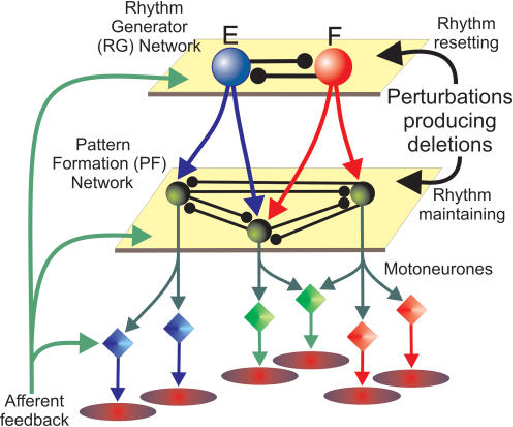
\includegraphics[width=0.80\textwidth,height=0.34\textheight,keepaspectratio]{rybak_cpg_circuit.pdf}
% ALT TEXT: A three-tier schematic shows the rhythm-generator half-centers
% above a pattern-formation network of interneuron populations that drive
% motoneuron pools and muscles, with green afferent-feedback arrows
% ascending to both levels.
\caption[Rybak two-level locomotor CPG concept]{Two-level CPG: rhythm generation (RG), pattern formation (PF), motor output, and afferent feedback. Reproduced from \citet[Fig.~1]{rybak_modelling_2006}.}
\label{fig:rybak_cpg_circuit}

\par\medskip

\centering
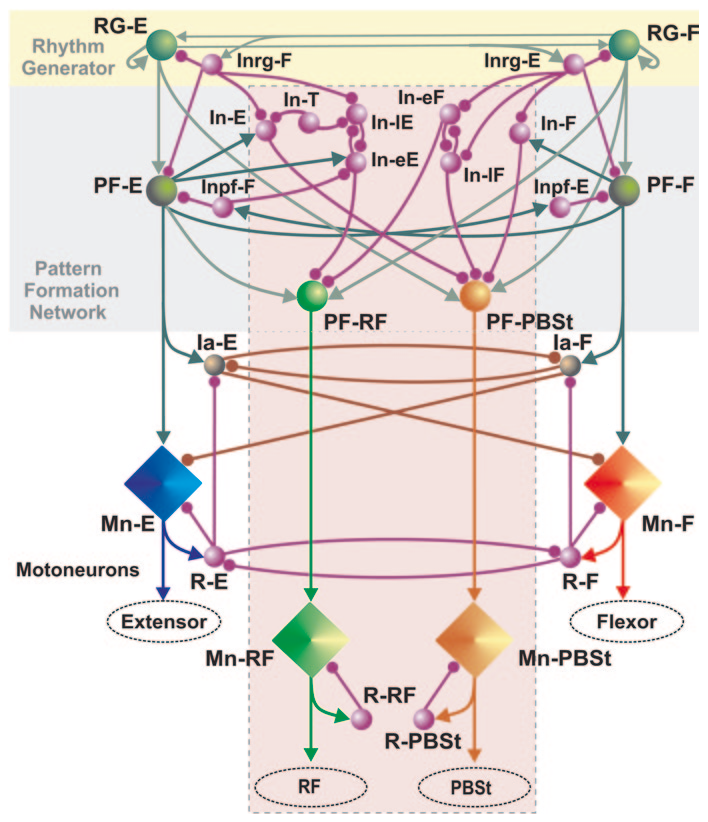
\includegraphics[width=0.88\textwidth,height=0.38\textheight,keepaspectratio]{shevtsova_spinal_circuit.pdf}
% ALT TEXT: A layered spinal circuit schematic shows rhythm-generator and
% pattern-formation populations above motoneuron and Renshaw-cell pools,
% with the two-joint-muscle extension for PBSt and RF outlined.
\caption[Shevtsova extended CPG model with two-joint-muscle circuits]{Extended CPG with pattern-formation and motor populations for the two-joint posterior biceps--semitendinosus (PBSt) and rectus femoris (RF). Reproduced from \citet[Fig.~5.8]{shevtsova_modeling_2016}.}
\label{fig:shevtsova_spinal_circuit}
\end{figure}



\section{Computational Neuroscience}\label{sec:bg_compneuro}

Computational neuroscience expresses hypotheses about neural circuitry as executable models. In conductance-based models, membrane voltages evolve through capacitance, leak, synaptic, and applied currents, and connections represent identifiable pathways \citep{nourse_sns_2023}. Model predictions can be compared with recordings or with responses to stimulation and pathway removal. This provides a way to test a proposed mechanism rather than infer it from a wiring diagram alone. Synthetic nervous systems use this approach to control physical and simulated bodies.

\section{Synthetic Nervous Systems}\label{sec:bg_sns}

For robots, these biological architectures can be implemented as synthetic nervous systems (SNSs): networks of conductance-based spiking and non-spiking neurons that are small enough to run in real time yet biologically grounded enough to be compared against animal data. The approach has been pursued most persistently by the insect-biorobotics lineage of the Quinn laboratory at Case Western Reserve University and by laboratories closely connected to it, my own included. Works in this lineage span several platforms: CPG-based neural control of a pneumatically actuated dog robot \citep{hunt_development_2017}, analytically designed dynamic neural networks for human balance control \citep{hilts_dynamic_2019}, the full-muscle rat hindlimb model and its moment-arm analysis \citep{young_analyzing_2019}, the two-layer CPG neuromechanical walker built on it \citep{deng_neuromechanical_2019}, which supplies this dissertation's controller architecture, and the Muscle Mutt quadruped, a canine-inspired BPA robot designed at my laboratory, the Agile and Adaptive Robotics Laboratory (AARL) at Portland State University, for synthetic nervous system control \citep{scharzenberger_design_2019}. Related controllers from the wider neuromechanical community include sensory-entrained CPG control of bipedal walking \citep{li_bipedal_2017}, inter-leg coordination analyses in stick-insect-inspired controllers \citep{nourse_analyzing_2019}, reinforcement-reflex hybrids in insects \citep{goldsmith_investigating_2021}, and adaptive hindlimb walking controllers \citep{schilling_adaptive_2022}.

The SNS-Toolbox \citep{nourse_sns_2023} makes such networks practical: it is an open-source Python package that simulates hundreds to thousands of spiking and non-spiking neurons in real time or faster, supports multiple software and hardware backends including GPUs and embedded platforms, and couples directly to physics simulators such as MuJoCo for musculoskeletal control. The field it serves is active and growing: the perspective review of \citet{szczecinski_perspective_2023} traces neuromorphic legged-locomotion control from its insect-robot beginnings through current platforms to open problems, and physical testbeds in this lineage now extend from insect-scale robots to a robotic cat hindlimb \citep{armstead_design_2025}.



\section{Neuromechanical Simulation}\label{sec:bg_neuromech}

Neuromechanical simulation, the coupling of a musculoskeletal model to a model of the neural controller that drives it, has advanced along three partially overlapping lines. The first line embeds reflex physiology directly into the controller. The muscle-reflex walking model of \citet{geyer_musclereflex_2010} demonstrated that positive force, length, and velocity feedback around each muscle, organized with simple interlimb coordination, is sufficient to produce self-stabilizing human-like walking dynamics and realistic muscle activations without any central pattern generator. That model became the reference point for a generation of reflex-based neuromechanical controllers, including the cat hindlimb models of Section~\ref{sec:bg_compneuro} \citep{markin_afferent_2010, shevtsova_modeling_2016} and their extensions. Hybrid work makes the complementarity of the two strategies explicit: \citet{haeufle_benefit_2018} combined feed-forward muscle activations with neuronal reflex feedback in simulated human walking and found that the robustness benefit of each depends on which muscle carries it.

The second line replaces hand-designed circuitry with machine learning. \citet{song_deep_2021} trained deep reinforcement learning policies on a physiologically realistic musculoskeletal model in OpenSim, reproducing human kinematics and muscle activations across locomotion tasks, with the learned policy re-usable for experiments that would be difficult in the laboratory. This approach inherits the fidelity of the musculoskeletal model but encodes control in opaque function approximations: the trained policy can reproduce behavior, but the individual ``neurons'' of the controller do not correspond to identifiable physiological circuits, so the class of scientific questions it can answer, such as lesions, deletions, and pathway stimulation, is narrower than its behavioral repertoire. Recent perspectives on predictive musculoskeletal simulation \citep{degroote_perspective_2021} place both learned and optimal-control approaches in the same frame: the models are mature, and the open problems are the cost of solving them and the biological interpretability of the control they find.

The third line, in which this dissertation sits, is biologically grounded synthetic nervous systems: controllers whose neurons and synapses are explicit, conductance-based, and mapped to identified physiological circuits, simulated at speeds sufficient for real-time robotics \citep{nourse_sns_2023}. Hierarchical CPG control is meanwhile spreading to bipedal-capable musculoskeletal models, including motor-module bipedal walkers \citep{ichimura_pathological_2019}, two-layer rhythm-generator and pattern-formation control of a musculoskeletal macaque model \citep{nishizaki_gait_2026}, and two-level CPG control of muscle-driven robotic hind legs \citep{fukuoka_autonomous_2021}, though always in simulation with generic musculature or on non-humanoid platforms; a two-layer SNS driving a custom-anatomy, artificial-muscle humanoid leg remains unclaimed. What distinguishes the present program from all three lines is the combination it attempts: an anatomically grounded controller (two-layer CPG with Ia, Ib, II, and contact feedback), a biomechanically validated pneumatic model (Chapter~\ref{ch:torque}), and an eventual physical robot.

\subsection{Simulation Tooling}\label{sec:bg_tools}

All three lines depend on a software substrate that is itself part of the method: musculoskeletal geometry too elaborate to integrate by hand, joined to neural models too large to wire by hand. The tools used in this dissertation, and the ones adjacent to it in the same ecosystem, are the following.

OpenSim \citep{delp_opensim_2007, seth_opensim_2018}, distributed through the SimTK (Simulation Toolkit) repository, provides the biomechanical modeling side: musculoskeletal models with detailed bone geometry, muscle routing, and force-generating properties, along with tools for analyzing moment arms and isometric torque. These models are approximations with known limits rather than exact anatomies: muscle paths are interpolations over discrete attachment and wrapping data, and near the ends of a joint's range the routed paths of sparsely wrapped muscles can bunch up or pass through bone, an interference documented within Gait2392-derived routings themselves \citep{bolen_bipedal_2019}. Their geometry is accurate for a purpose, namely moment arms and torque predictions over the functional range of motion, and that is the standard against which the robot model of this program is compared. The same SimTK infrastructure hosts SCONE, an open-source package for predictive simulation and optimization of neuromuscular control of biological motion \citep{geijtenbeek_scone_2019}. AnimatLab \citep{cofer_animatlab_2010} provides a graphical environment in which physical bodies and synthetic neural systems are constructed and co-simulated; the AARL's prior walker (Section~\ref{sec:prior_walker}) was built in it. MuJoCo \citep{todorov_mujoco_2012} provides the physics-engine side: fast, accurate simulation of rigid-body dynamics with contacts, along with muscle-like actuators that include activation dynamics. MyoConverter bridges the biomechanical and physics-engine worlds by converting OpenSim musculoskeletal models to MuJoCo format with optimized muscle kinematics and kinetics \citep{caggiano_myosuite_2022, wang_myosim_2022}. Combined with the SNS-Toolbox's MuJoCo backend \citep{nourse_sns_2023}, I used these tools to convert the laboratory's modified OpenSim leg model to MuJoCo and couple it to a synthetic nervous system, a pipeline assembled and evaluated in Chapter~\ref{ch:sns}. Simulation speed is the practical enabler: a single overnight run can sweep thousands of parameter combinations or execute hundreds of simulated gait cycles per condition, throughput that no human-subject or animal protocol could match, and that transforms lesion and stimulation studies from bespoke demonstrations into statistically powered experiments.

\section{Testing Neuromechanical Hypotheses on Robots: The Ethical Case}\label{sec:bg_ethics}

The experiments this research program is designed to enable, including deleting a muscle from a limb, blocking a sensory pathway, lesioning part of a rhythm generator, and applying tonic stimulation to spinal circuits, cannot be performed on healthy humans. Invasive intervention on the human neuromuscular system is limited to clinical populations, is tightly constrained by ethics review, and permits neither the within-subject control nor the reversibility that neuromechanical hypotheses demand. The same experiments in animals also carry real moral cost, and their justification is governed by the Three Rs framework: replacement of animal subjects with non-animal methods, reduction of the numbers required, and refinement of the remaining procedures \citep{russell_principles_1959, tannenbaum_russell_2015}. A robot that implements a validated neuromechanical hypothesis is precisely such a replacement method: every deletion, lesion, and stimulation experiment that runs on the synthetic nervous system is an experiment that does not require a living subject, and the robot population can be duplicated exactly, so that ``subjects'' are statistically identical across conditions, a form of reduction no breeding colony can offer. Refinement follows as well: the failure modes of these experiments damage hardware, not tissue.

Figure~\ref{fig:decerebrate_cat} shows what that accounting leaves out. The image is a frame from footage of a real decerebrate-cat experiment, the class of preparation on which the field's understanding of spinal locomotion has been built since its beginnings \citep{brown_intrinsic_1911, decerebrate_cat_footage}: a living cat, its forebrain disconnected by a brainstem transection, walks on the treadmill because the neurons distal to the laceration are still living, still connected, and still firing action potentials. The published record of this work is drawn almost exclusively in schematic, labeled boxes for half-centers and color-coded reflex arcs that are honest about the circuitry and silent about the animal. The figure is included as the counterweight, documenting what the experiments looked like, and therefore what a replacement method stands in for.

\begin{figure}[htbp]
\centering
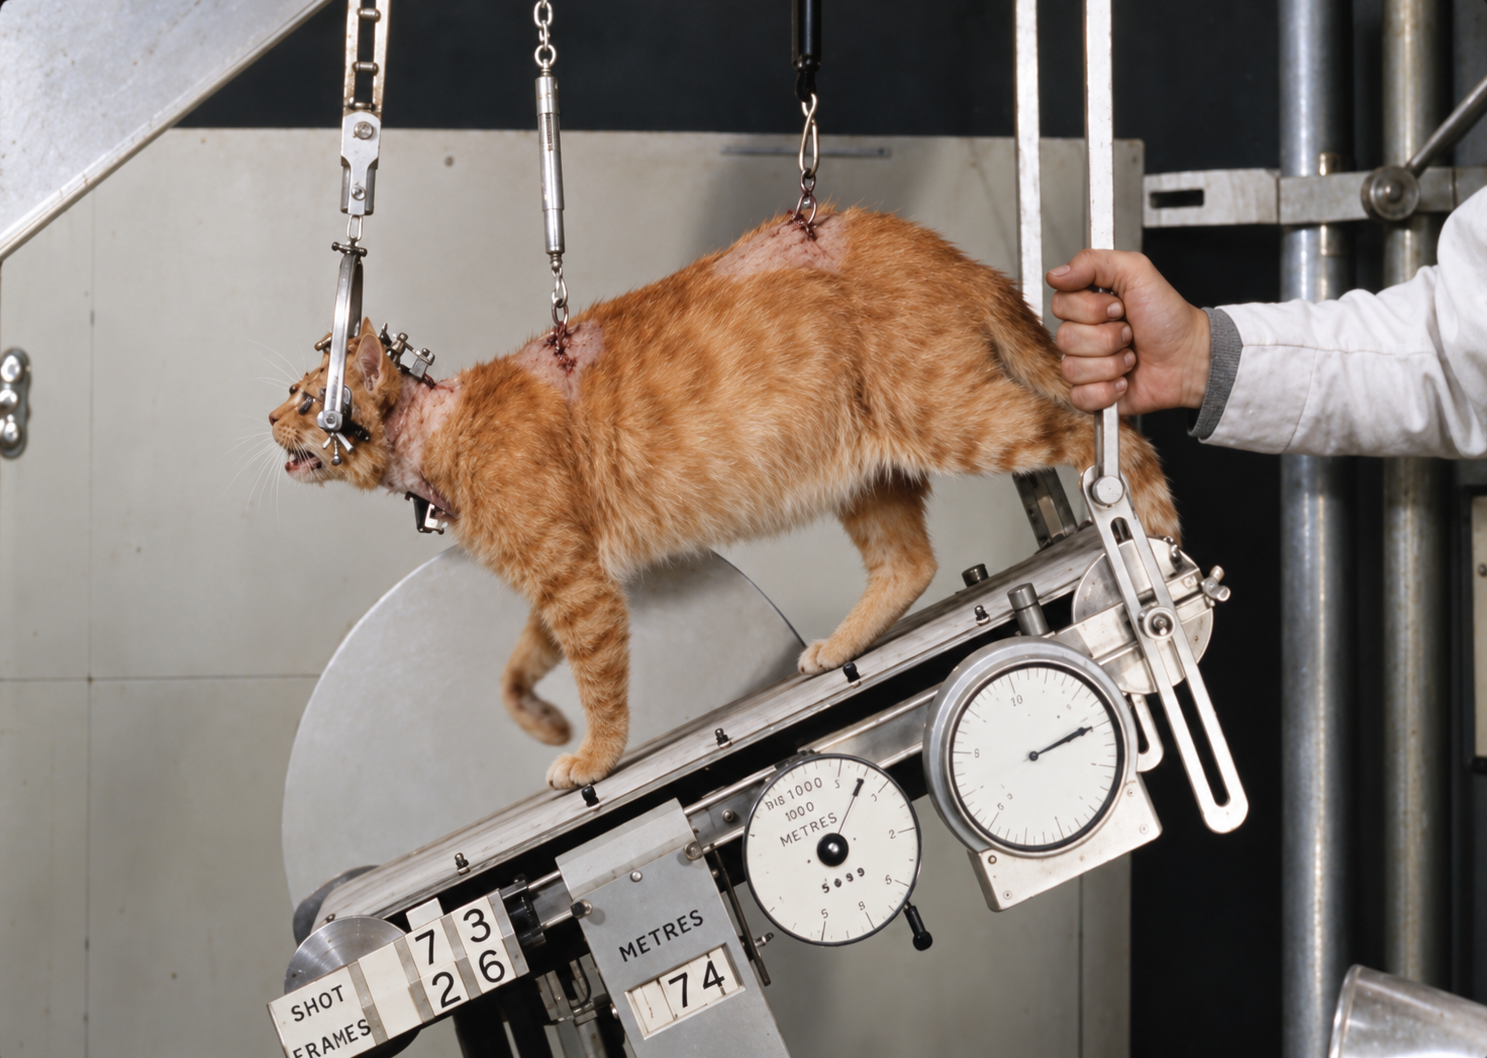
\includegraphics[width=0.82\textwidth]{decerebrate_cat_colorized.png}
% ALT TEXT: A cat held in a stereotactic head holder with skull clamps and a
% fixation pin beside the eye orbit stands on a moving treadmill belt in a
% laboratory, supported by rigging, walking.
\caption[Decerebrate-cat treadmill experiment]{Restored and colorized frame from archival footage of a decerebrate-cat treadmill experiment \citep{decerebrate_cat_footage}.}
\label{fig:decerebrate_cat}
\end{figure}

The procedures behind that record are documented in films that remain publicly available. A \qty{50}{\minute} classroom recording posted by the UTHealth Houston School of Dentistry first shows an intact cat playing with its handler, righting itself when lowered and placing its paws accurately on the edge of a table, and then documents the decerebration performed for the class \citep{utherst_decerebrate_2025}: the animal is anesthetized with open-drop ether, more than the horse in the same demonstration series received, the carotid arteries are ligated and a tracheal cannula installed, and the skull is opened with a trephine before the brainstem is transected between the superior and inferior colliculi. The treadmill preparations that established locomotor neurophysiology are likewise preserved in the historical literature: \citet{stuart_reflections_2007} reproduce the arrangement of the high-decerebrate cat treadmill experiments, with electromyographic recording from the hindlimb muscles, from the original Russian-language reports \citep{severin_1967}.

The honest accounting is murkier than the Three Rs framing alone suggests, because the models a robot implements are themselves products of animal experimentation. The half-center organization, the two-level rhythm and pattern architecture, and the length, force, and load signaling of the afferents were each established in preparations like the ones described above \citep{brown_intrinsic_1911, severin_1967, rybak_modelling_2006}, and the databases of afferent properties that parameterize sensory feedback are compiled from animal recordings \citep{bolen_sensory_2023}. A synthetic nervous system therefore replaces future experiments; it does not replace, and cannot repay, the animal work on which its architecture is built. Recognizing this inheritance sharpens rather than undermines the case for robotic subjects: the knowledge purchased at that cost is precisely what makes a robotic replacement scientifically meaningful, and the robot is the instrument that keeps that knowledge productive without adding to the ledger.

For a robot to serve as a replacement subject, however, it must first earn standing as a scientific model. Webb's influential analyses of bio-robotic methodology \citep{webb_robots_2001, webb_robots_2002} argue that a robot is a good model of biological behavior when the mechanism it implements is tested at the same level of organization as the target phenomenon, matching dynamics, control structure, and sensory ecology rather than surface appearance. The validation chain of this dissertation is constructed to that standard: the actuator force model is validated against bench data (Section~\ref{sec:results_force}), the joint torque model against isometric measurements and human torque envelopes (Section~\ref{sec:results_torque}), and selected controller responses are compared with published tonic stimulation and deletion phenomena \citep{selionov_tonic_2009, rybak_modelling_2006}, the verification step that precedes locomotion tuning in this program. Only then can a robot experiment be read as evidence about the hypothesized biological circuit rather than about the robot.

The argument is ultimately bidirectional, completing the loop described in Section~\ref{sec:project}. Experiments that are unethical, impractical, or statistically unreachable in humans and animals become routine on the robot; the resulting insights into neuromechanical control feed back into biology, into the design of the next robot iteration, and directly into prosthetic and orthotic devices that face the same problem of controlling muscle-like actuators for human users, whose central pattern generator controllers are an active topic in lower-limb exoskeleton research \citep{duan_gait_2024, pery_benchmarking_2026}. The ethical case and the scientific case are the same case: the robot is the instrument that makes these experiments possible.
